\documentclass{report}
\usepackage{amsmath}
\usepackage{tabularx}
\usepackage{graphicx}
\usepackage{dirtree}
\usepackage{listings}
\lstdefinestyle{Python2}
{
	language=Python,
	literate = *{\ \ }{\ }1, %replaces each occurence of two consecutive spaces by one
}


\begin{document}
	
\title{Clay-Wolkin Fellowship ISP: Mid-Year Report}
\author{Nick Draper, Christine Goins, Kaveh Pezeshki, Zunyan Wang, Nancy Wei}
\date{November 2017}
\maketitle

\tableofcontents

\begin{abstract}
	\label{abstract}
\end{abstract}

\chapter{Introduction}
	For the 2017-2018 term the Clay-Wolkin fellows will develop an image signal processor (ISP) specifically for object recognition by convolutional neural networks. The team is working with guidance from Reduced Energy Microsystems, and will design the ISP according to their specifications. Commercial ISPs are highly proprietary and open source ISPs are not designed for machine learning in particular. Thus, the project presents an interesting area of research and application. 
\chapter{Project Goals}
	The overall objective of the project is to develop an ISP suitable for object recognition by convolutional neural networks.
	\section{Constraints}
	There are several critical constraints for the ISP, as defined by the team and Reduced Energy Microsystems:
	\begin{itemize}
		\item The ISP must achieve image recognition rates comparable to images produced by commercial ISPs. The metric for recognition success is determined by the team. 
		\item The ISP will be made open source at the end of the project.
	\end{itemize}
	\section{Hardware Specification}
	The ISP inputs are defined below:
	\begin{itemize}
		\item Parameters specific to the camera sensor:
		\begin{itemize}
			\item Bayer filter array pattern (RGGB, BGGR, GBRG, or GRBG)
			\item Color conversion matrix 
		\end{itemize}
		\item Number of bits per pixel
		\item Desired file format of output (JPEG, PNG, or TIFF)
	\end{itemize}
	The ISP will output processed images in the desired file format. 
	
\chapter{Background Information}
	\section{Image Signal Processing}
	Image signal processing is a fundamental component of all modern camera systems. A digital camera sensor outputs light intensity values for its sub-pixel array: blue, red, and green sub-pixels typically arranged in a Bayer pattern, with an uneven distribution of sub-pixels sensitive to each color\footnote{http://www.siliconimaging.com/RGB\%20Bayer.htm}. The role of an image signal processor, or ISP, is to decode the sub-pixel intensity matrix sent in scanlines from the image sensor, calculate the color, as per the SRGB\footnote{https://www.w3.org/Graphics/Color/srgb}, AdobeRGB\footnote{https://www.adobe.com/digitalimag/pdfs/AdobeRGB1998.pdf}, or other color standard, of each set of sub-pixels, providing gamma (image brightness), white balance (color temperature), and other image corrections necessary during the conversion process.
	
	ISP pipelines range from simple, with only the bare minimum demosaicing (interpreting sub-pixel arrangement) and color conversion steps, to complex, with features such as denoising and chromatic abberation correction. Through the team's project, the team will determine necessary image signal processing steps to optimize image classification performance.
		
	\section{Image Recognition via CNN}
	
\chapter{Microarchitecture Specifications}


\chapter{Examining the DCraw Conversion Pipeline}
\section{Introduction}
\subsection{Overarching Goals}
The end goal of this project is to create an ISP optimized for neural network image classification. However, examining each of the wide variety of algorithms for different image conversion steps in the context of image classification presents a challenge beyond the time available to the team. DCraw, an open-source software application for RAW file image conversion, implements many of these algorithms in a user-friendly format. By examining DCraw image output performance in image classification, the team would be able to identify image conversion algorithms optimized for image classification. The team aimed to produce an ISP capable of outperforming an integrated DSLR ISP in image classification.

\subsection{Prior Analysis}
The team had initially tried to create custom algorithms for image conversion. Reading in raw pixel data from a Canon t30i, simple image conversion algorithms were used to create a .png file that could be analyzed by neural networks. Code for these algorithms is available in section \ref{pipelinecode}. A metric, described in section \ref{metric}, provided a numerical value of image classification performance. Tests on the second image set, described in sections \ref{test1} and \ref{test2}, illustrated the inadequacy of the team's initial pipeline, with Demosaicing and Demosaicing (2) indicating different demosaicing algorithms. Image classification data can be seen in Figure \ref{inittests}.

\begin{figure}[!htb]
\label{inittests}
\caption{Initial Custom Pipeline Testing Data}
\begin{tabular}{lc}
	Processing Steps & Classification Rate \\
	\hline
	Camera ISP & 0.94 \\
	Demosaicing & 0.60 \\
	Demosaicing (2) & 0.68 \\
	Color Correction, Demosaicing & 0.49 \\
	Color Correction, Demosaicing (2) & 0.49 \\
	White Balancing, Demosaicing & 0.49 \\
	White Balancing, Demosaicing (2) & 0.50 \\
	Brightness, Demosaicing & 0.45 \\
	Brightness, Demosaicing (2) & 0.40 \\
	Brightness, Color Correction, Demosaicing & 0.45 \\
	Brightness, Color Correction, Demosaicing (2) & 0.45 \\
\end{tabular}
\end{figure}

\subsection{RAW Conversion}
As preliminary algorithm implementation provided inadequate image classification performance, the team examined commercial RAW image converters. RAW images essentially provide the same output as a camera module as will be used with the final ISP: they provide intensity values for every sub-pixel in the camera Bayer array. Therefore RAW image converters, which output a processed .JPG, .TIFF, .PNG, or other filetype with a RAW file as input, include a superset of the image processing steps required in the team's final ISP. 

Many RAW image converters also provide enough user control to select algorithms and algorithm parameters for each image processing step. Therefore, by examining image classification performance of different algorithm and parameter values within a RAW converter, the team can determine suitable algorithms without implementing each algorithm to be tested in a custom software pipeline.

Typically, applications such as Adobe Photoshop, Adobe Lightroom, or other commercial packages are used to process RAW photos. However, these packages do not provide the user the ability to select individual conversion algorithms or to view algorithm source code. Therefore they were unsuitable for the team's conversion goals. However, open-source RAW conversion applications also exist, such as UFraw\footnote{http://ufraw.sourceforge.net/}, Mogrify\footnote{https://www.imagemagick.org/script/mogrify.php}, and ImageMagick\footnote{https://www.imagemagick.org/script/index.php}. These tools provide user-friendly wrappers for DCraw\footnote{https://www.cybercom.net/~dcoffin/dcraw/}, which allows direct user control of algorithm options and parameter values. Additionally Research on the image quality - image classification performance correlation already exists\footnote{https://arxiv.org/pdf/1604.04004.pdf}, and indicates that image deviations that can be compensated for in post-processing have substantial impact on recognition rate, showing that algorithmic improvements as seen in software processing pipelines can significantly enhance image classification performance. The team therefore decided to proceed to test image optimization via UFraw and DCraw.

\subsection{Testing Overview}
The team had two goals in testing the DCraw conversion pipeline. First, to determine whether DCraw can provide adequate classification rates across a variety of image conditions. Second, to test classification rates across various algorithms provided by DCraw. Provided that DCraw produces adequate classification rates, minimizing the number and complexity of steps in the image conversion pipeline will provide a simpler ISP design, reducing production cost and potentially increasing clockspeeed and therefore throughput.

The team will accomplish the first test through manipulating six parameters in the UFraw wrapper for DCraw: color temperature, green component, gamma, exposure, saturation, and black point. It was possible to use UFraw as it only provides a wrapper for DCraw: UFraw parameter values are translated into DCraw arguments, and UFraw provides a convenient front-end with features such as batch image processing. For each parameter, sets of images will be generated from a single RAW image set with a single parameter value sampled multiple times across the parameter domain. This process was repeated for each of the six parameters. Once images have been generated, recognition rate will be tested as described in sections \ref{test1} and \ref{test2} for each image set to determine if the parameter value provides adequate recognition.

The team will generate image sets for each DCraw algorithm option in order to determine unnecessary pipeline steps, or to determine whether simpler conversion step algorithms are adequate. Images sets would be tested via the same method as above, and a 1-2\% decrease in classification rate in exchange for a simpler pipeline was deemed acceptable.

\section{Hardware and Software}

\subsection{Test Server}
All image set generation and testing was done on a team member's home server: an HP Microserver G8\footnote{https://www.hpe.com/h20195/V2/Getdocument.aspx?docname=c04128132}, with an Intel Celeron G1610T\footnote{https://ark.intel.com/products/71074/Intel-Celeron-Processor-G1610T-2M-Cache-2\_30-GHz} and 4GB of ECC DDR3 RAM. All team files were stored on a single 3TB hard drive.
\subsection{Software Setup}
\label{ssetup}
The server ran Ubuntu Server 16.04. Directory structure for the project folder was as follows:

	\dirtree{%
		.1 ~/cw.
		.2 autogen.py.
		.2 tensorflow.
		.3 <tensorflow installation>.
		.2 tensorflow\_loader.
		.3 config.txt.
		.3 readme.txt.
		.3 image\_loader.py.
		.3 metric\_calc.py.
		.3 tensorflow\_parser.py.
		.2 images.
		.3 images.
		.4 <image folders>.
		.4 ufraw\_param.
		.4 ufraw\_pumpkin.
		.4 ufraw\_cat1.
	}

	autogen.py was a custom script that generated directory creation commands as well as elements of a configuration file for tensorflow operation. The tensorflow operation scripts are within the tensorflow\_loader directory. After defining the location of any image sets to process, location of the tensorflow directory, a filename for recognition statistics, and whether to print image statistics to the terminal in the configuration file config.txt, running metric\_calc.py automates the tensorflow image classification process. More details on usage of these scripts are available in sections \ref{test1} and \ref{test2}.
	
	Tensorflow was installed with CPU support only as shown in the official installation guide\footnote{https://www.tensorflow.org/install/install\_linux}, set up within virtualenv. The image recognition tutorial\footnote{https://www.tensorflow.org/tutorials/image\_recognition}, setting up the image classification network Inception-V3 on Tensorflow was followed to produce the final Tensorflow system. Converted image sets were stored throughout the project directory, but generally, image set 1 derivatives were stored in in cw/ufraw\_cat1, image set 2 derivatives in ufraw\_param, and image set 3 derivatives in ufraw\_pumpkin.



\section{Image Collection}
\subsection{Image Collection Goals}
As the final ISP was expected to produce images over a variety of sensor specifications, lighting conditions, subject speed, and other parameters, the team needed to provide representation of a variety of image conditions within the image sets. Additionally, for the recognition metric described in section \ref{metric}, it was necessary to choose subjects for which there was adequate granularity within the Inception-V3 training set. Inception-V3 was trained on the ImageNet database\footnote{http://www.image-net.org/}, which contains a large number of photos of feline species. Hence a subject of `cat' provided acceptable granularity.

\subsection{Image Set 1}
The initial keyword chosen was 'cat'. This was due to the large proportion of cats and related cat breeds in the ImageNet database\footnote{http://image-net.org/synset?wnid=n02127808}, as well as similar quadripedal animals. These characteristics of the ImageNet database would provide a large amount of granularity in the Inception-V3 output. This granularity would allow for a greater level of fine-tuning in ISP pipeline optimization.

There is an animal shelter near Harvey Mudd College, Priceless Pet Rescue\footnote{http://pricelesspetrescue.org/}. The initial image set was composed of 83 RAW images of cats and dogs under CFL-lit conditions. There were 32 dogs and 51 cats in this image set. Images were taken in simultaneous RAW-JPG mode with a Canon Rebel t30i, at 5184x3465 pixel resolution.

Images were also taken of dogs and other shelter animals to provide a negative reference. A few example images, processed through the camera pipeline, can be seen in Figure \ref{set1}.

\begin{figure}[!htb]
	\begin{center}
		\caption{Example Images from Set 1}
		\label{set1}
		\includegraphics[width=8cm]{set1_cat1.JPG}
		\includegraphics[width=5cm]{set1_cat2.JPG}
		\includegraphics[width=5cm]{set1_dog.JPG}
	\end{center}
\end{figure}

\subsection{Image Set 2}

Realizing that a set of images taken under optimal, well-lit, conditions are likely not representative of images in potential applications of the team's ISP, the team elected to take another set of images at the Priceless Pet Rescue. There were 102 images of cats and 58 images of dogs in this image set for a total of 160 images. Pictures were again taken in simultaneous RAW-JPG mode on a Canon Rebel t30i, except with unoptimal ISO, shutter speed, camera shake, and other parameters.

As before, non-cat images of dogs and other animals were included in the set. Example images can be seen in Figure \ref{set2}. The image quality degradations are immediately clear from these examples.

\begin{figure}[!htb]
	\begin{center}
		\caption{Example Images from Set 2}
		\label{set2}
		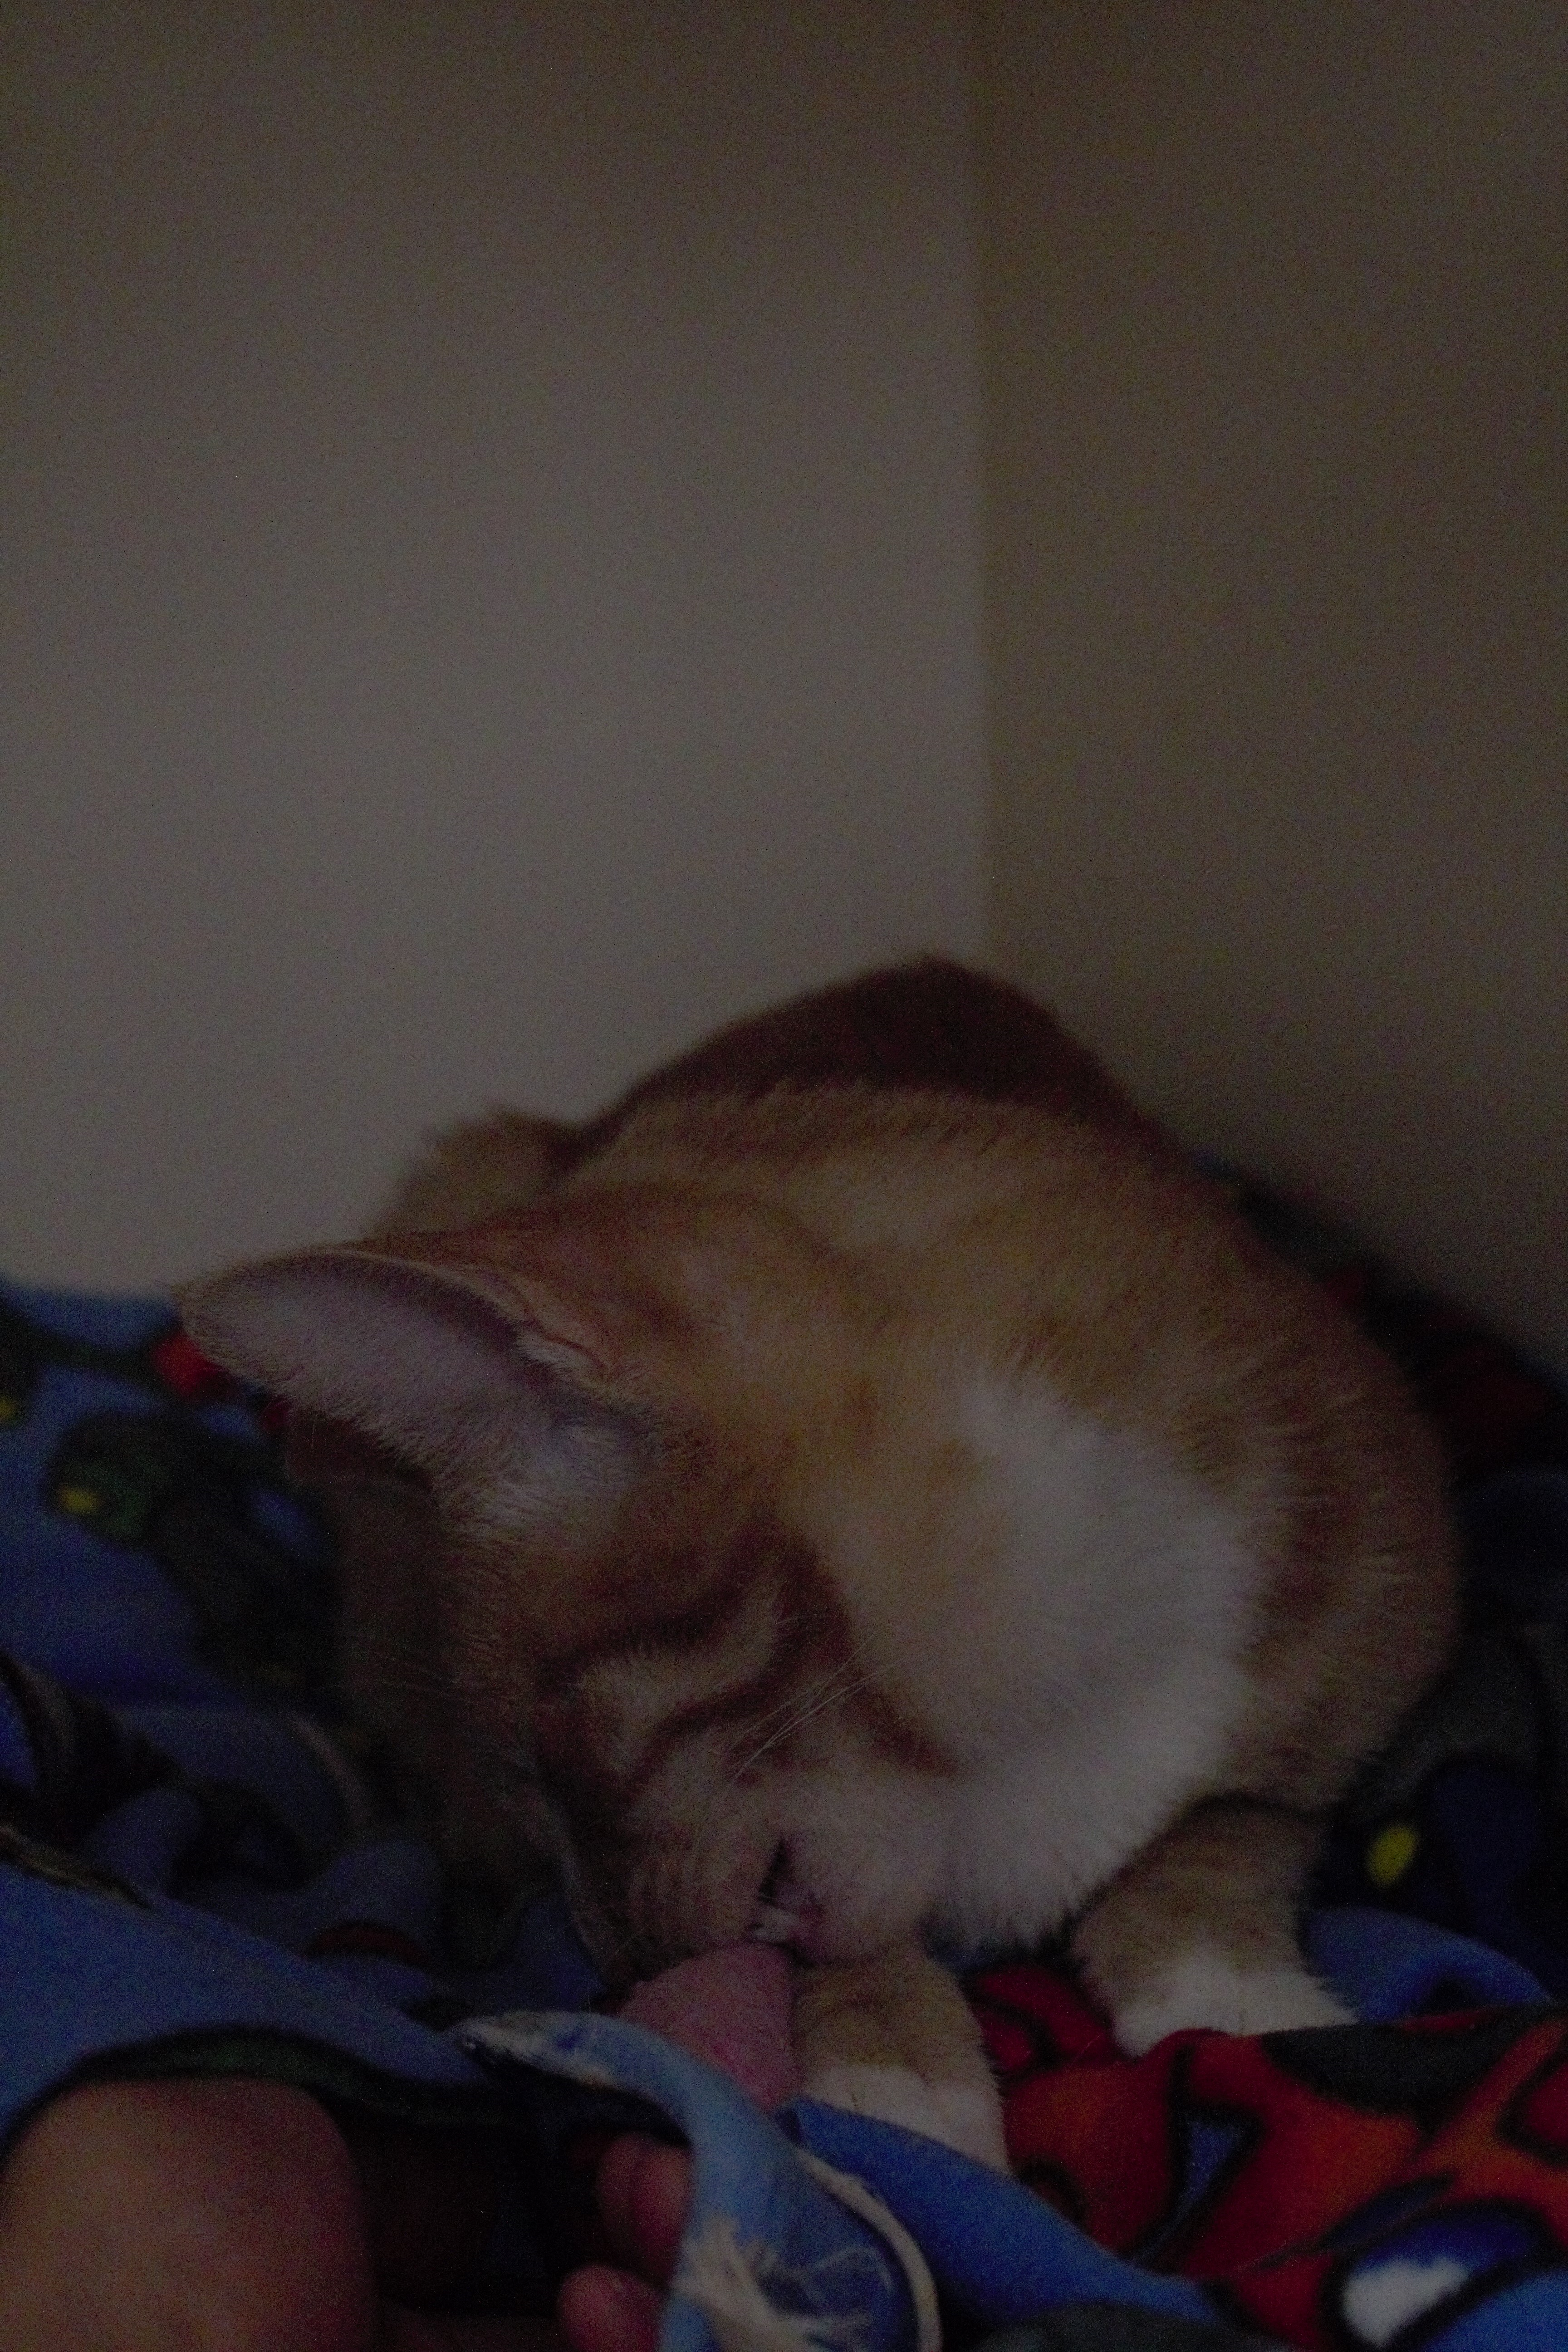
\includegraphics[width=5cm]{set2_cat1.PNG}
		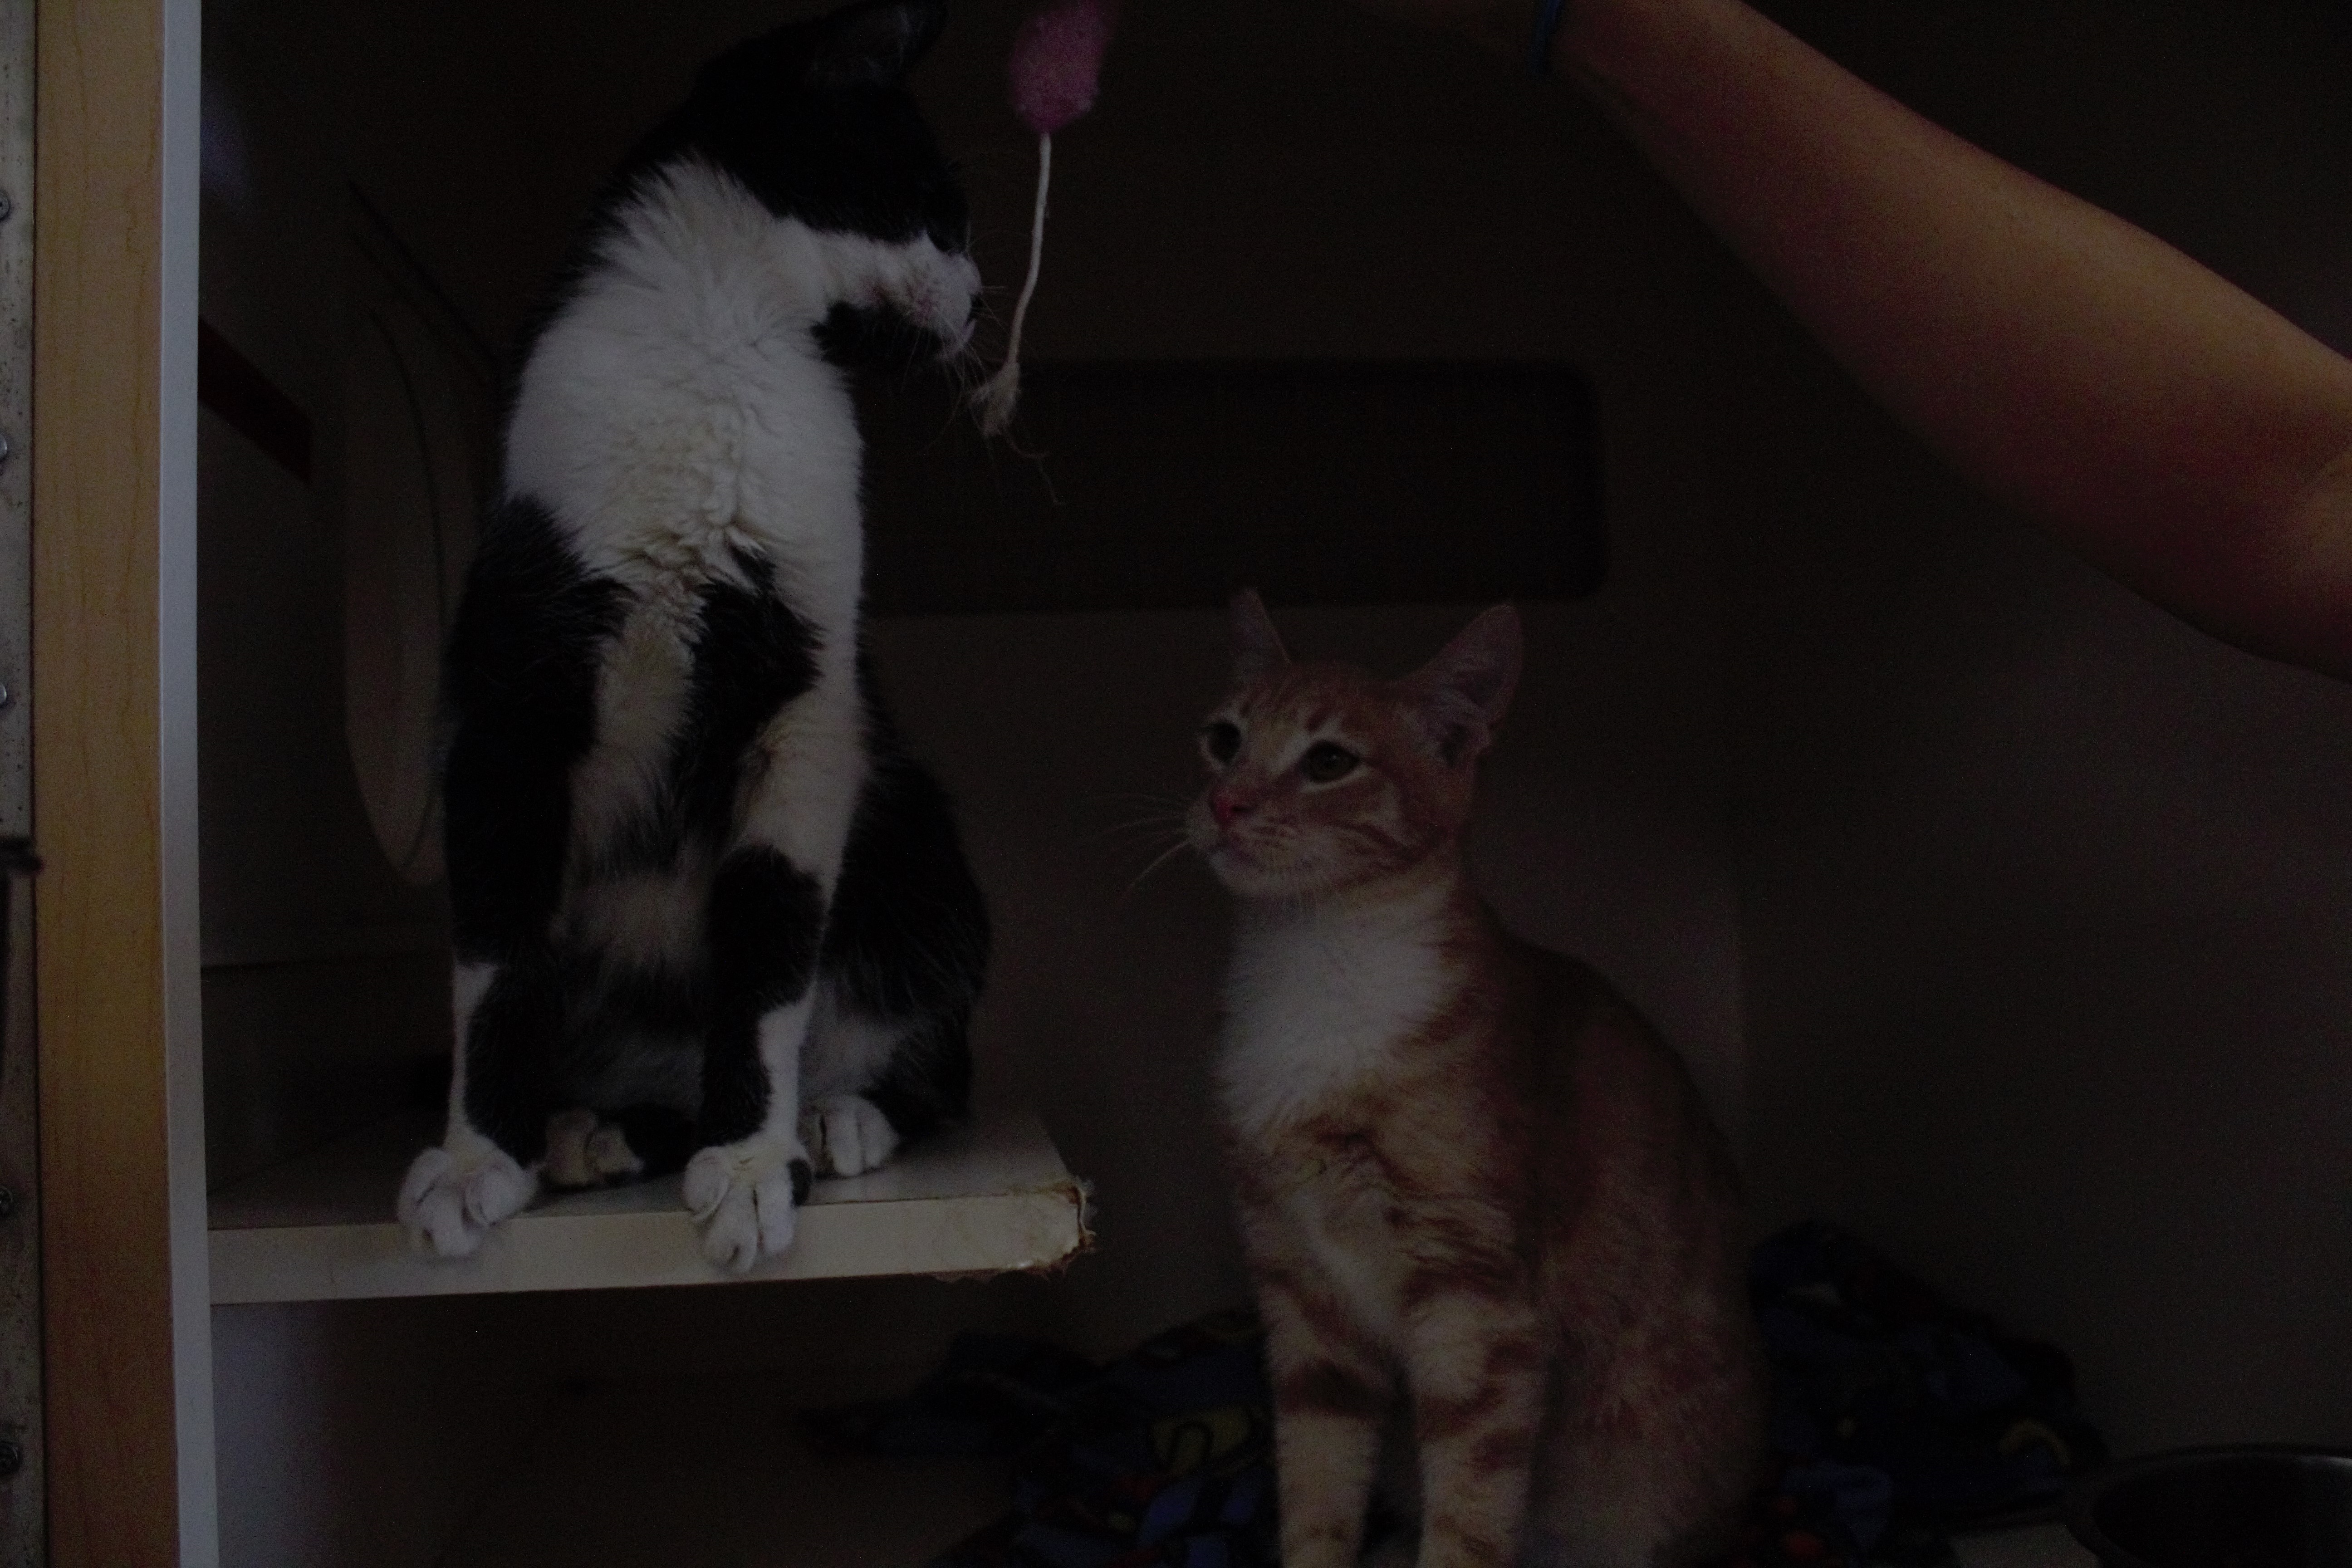
\includegraphics[width=8cm]{set2_cat2.PNG}
		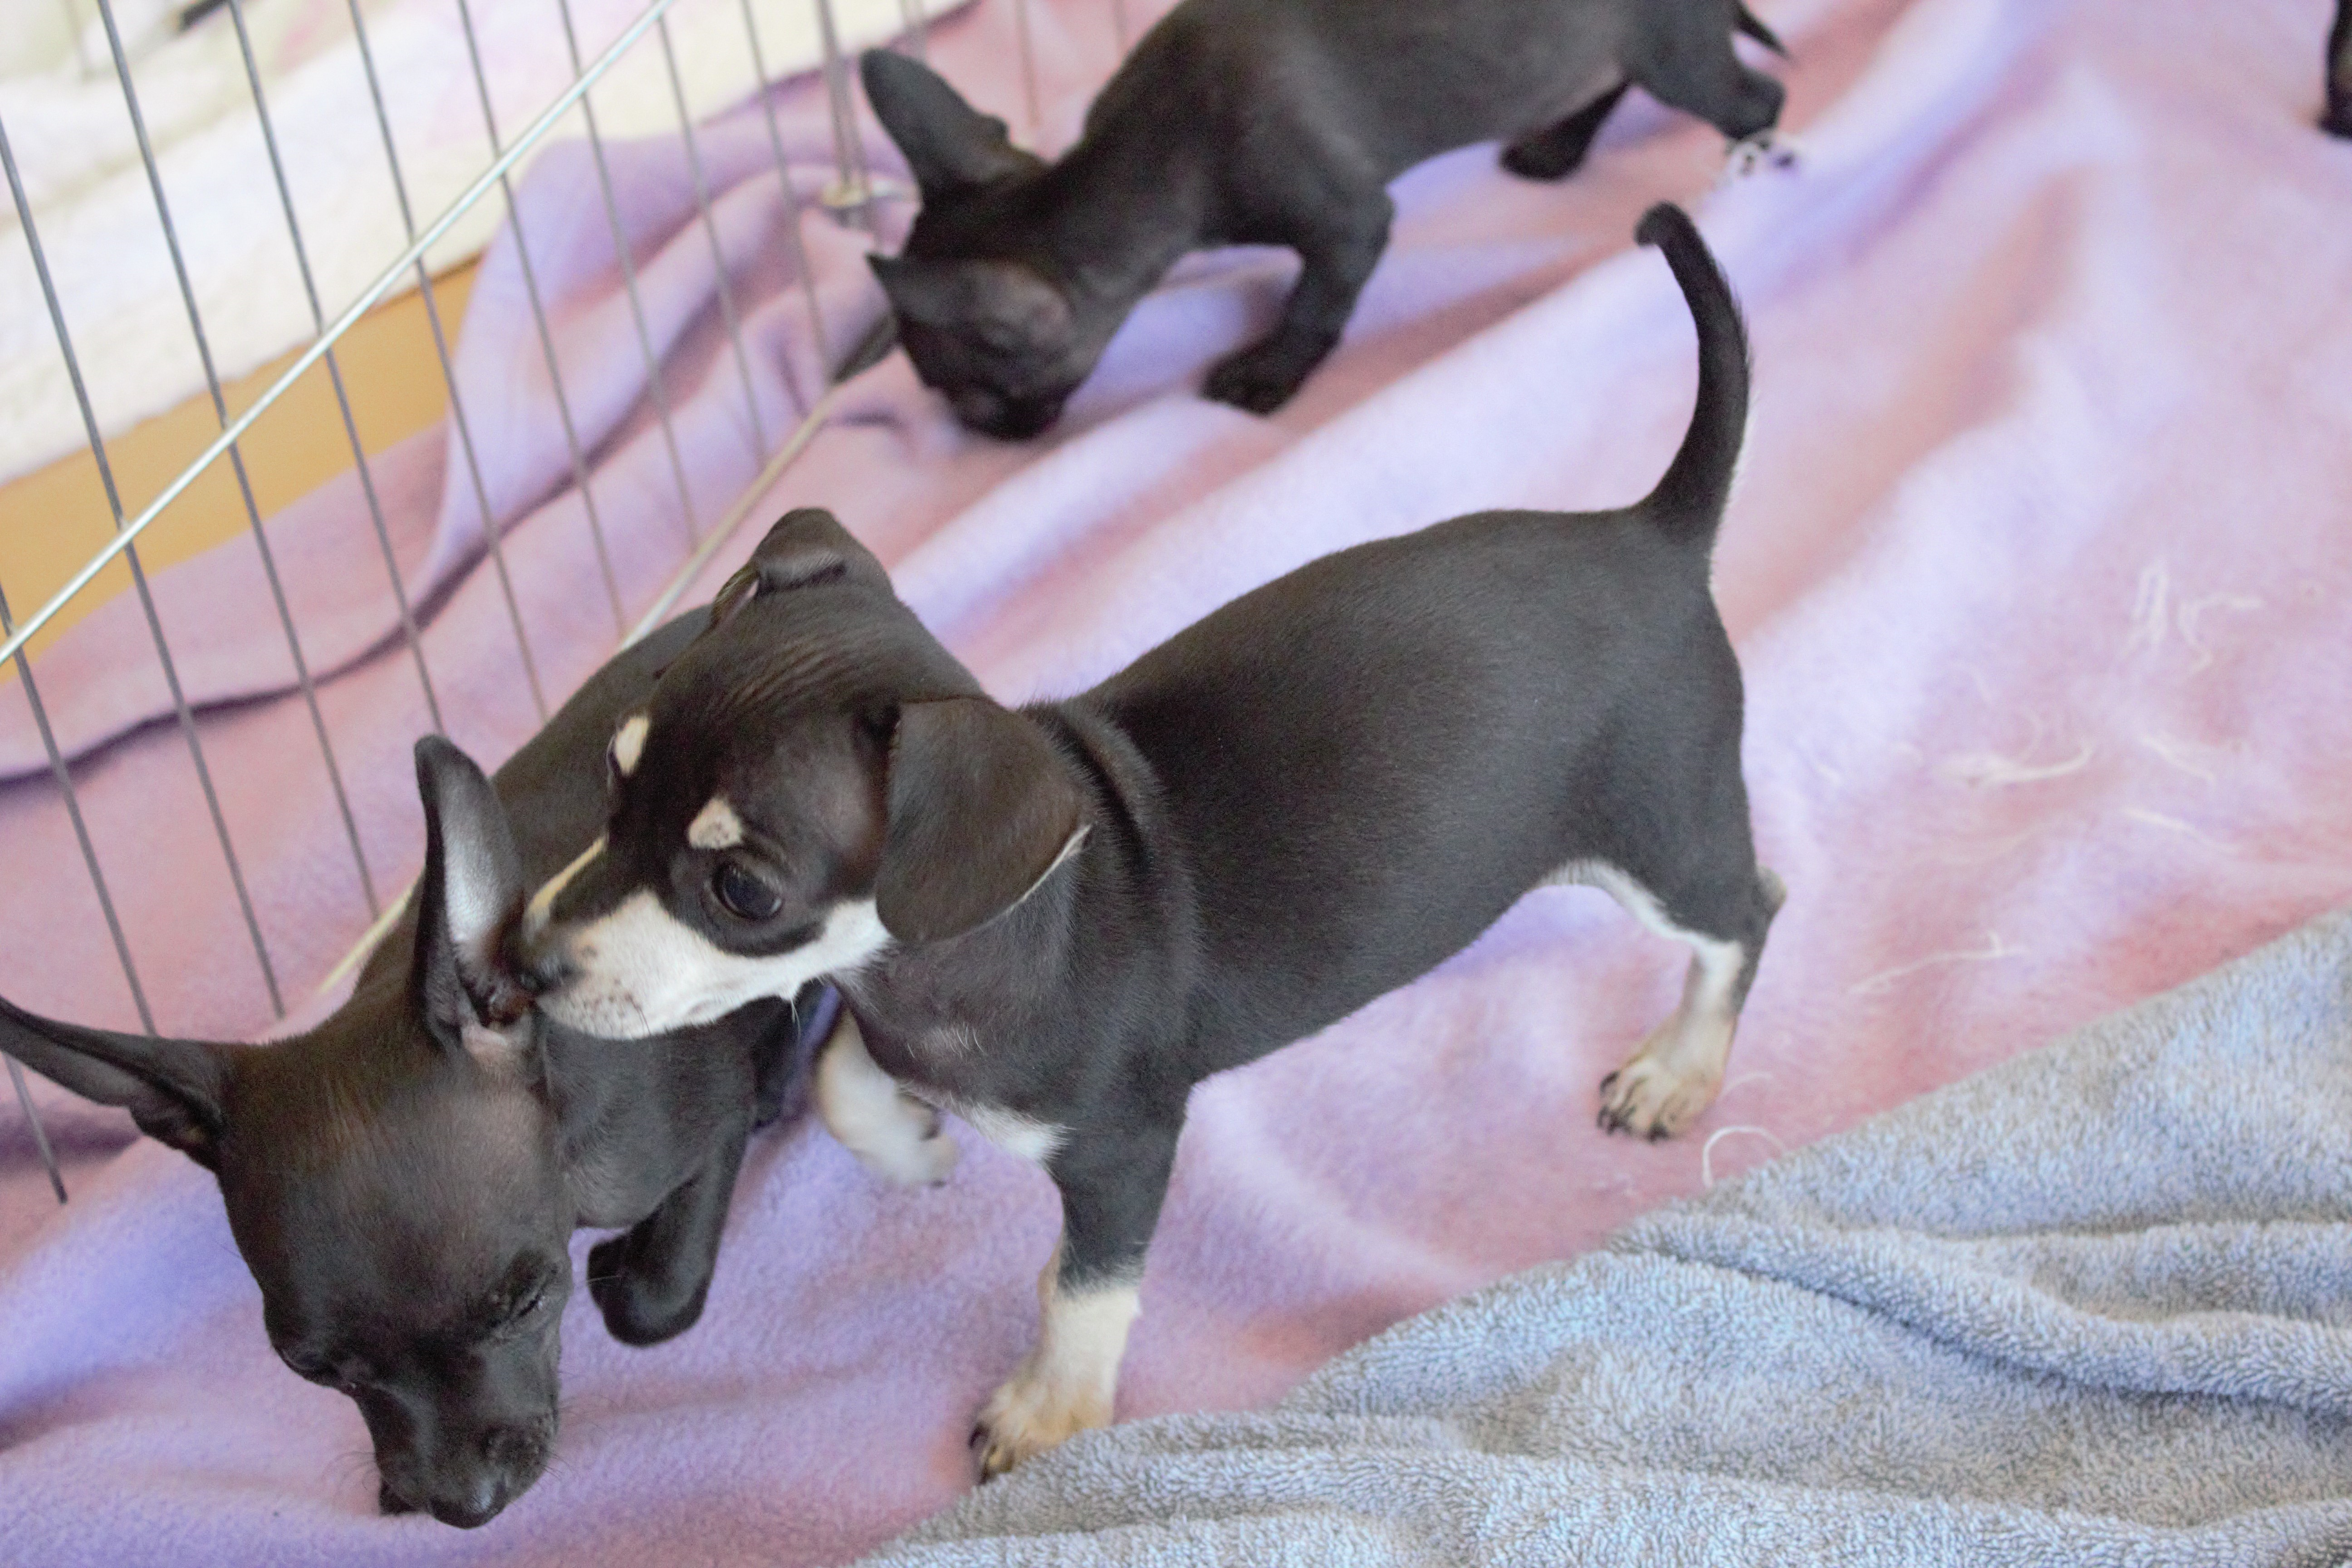
\includegraphics[width=8cm]{set2_dog.PNG}
	\end{center}
\end{figure}		

\subsection{Image Set 3}
The third and final image set was taken with an unrelated subject --squash-- to help ensure that identification rates were not directly correlated with the cat subject. This image set was taken in simultaneous RAW-JPG mode on a Canon Eos 80D, under outdoor nighttime conditions. Negative samples were of street signs, food products, and other similar objects. There were 29 images of squash of the 102 images in this set. As with the cat subject, the ImageNet database provided adequate granularity with a squash subject.

As before, example images are given in Figure \ref{set3}.

\begin{figure}[!htb]
	\begin{center}
		\caption{Example Images from Set 3}
		\label{set3}
		\includegraphics[width=8cm]{set3_pumpkin1.JPG}
		\includegraphics[width=8cm]{set3_pumpkin2.JPG}
		\includegraphics[width=8cm]{set3_other.JPG}
	\end{center}
\end{figure}	

\section{Test Methodology}
\subsection{Recognition Metric}
\label{metric}
In order to judge the efficacy of image optimization, it was first necessary to establish a metric. Focusing on the Inception-V3 image recognition model, trained on ImageNet\footnote{http://www.image-net.org/} and implemented on Google's Tensorflow CNN framework\footnote{https://www.tensorflow.org/}, the team decided on a simple binary calculation scheme.

Each image set would focus on a specific keyword, with images of the keyword's subject as well as a distribution of images of related and unrelated entities. The metric would be equal to:

\footnotesize
\hspace{-1.5cm}
\begin{equation*}
\text{metric}=\frac{\text{Number of correct top-5 positive identifications}}{\text{number of images}} + \frac{\text{Number of correct negative identifications}}{\text{number of images}}
\end{equation*}
\normalsize

\subsection{Maximizing DCraw Recognition}
\label{test1}
The first DCraw pipeline test tested maximum image classification images of RAW files converted by the UFraw wrapper over a variety of parameter values across all three image sets. The team first chose the set of values across the six different parameters to test. For each value, only one specific parameter was set: the other five parameters were left at their default values. Descriptions of each parameter can be seen in the UFraw man page\footnote{http://ufraw.sourceforge.net/Guide.html}, and a table of the parameters chosen by the team are available in Figure \ref{ufraw_settings}.

\begin{figure}[!htb]
	\begin{center}
		\label{ufraw_settings}
		\caption{UFraw Parameter Test Settings}
		\begin{tabular}{cccccc}
			temperature & green & gamma & exposure & saturation & black-point \\
			\hline
			2700 & 0.2 & 0.1 & -3 & 0 & 0 \\
			3000 & 0.6 & 0.3 & -2 & 1 & 0.2 \\
			3300 & 1 & 0.5 & -1 & 2 & 0.4 \\
			3600 & 1.4 & 0.7 & 0 & 3 & 0.6 \\
			3900 & 1.8 & 0.9 & 1 & 4 & 0.8 \\
			4200 & 2.2 && 2 & 5 & 1 \\
			4500 &&& 3 & 6 & \\
			4800 &&&& 7 & \\
			5100 &&&& 8 & \\
			5400 &&&&& \\
			5700 &&&&& \\
			6000 &&&&& \\
			6300 &&&&& \\
		\end{tabular}	
	\end{center}
\end{figure}

For each image set, the converted image output directory was specified in the output dir variable of autogen.py. Image conversion commands were generated by calling concatCommands() on the output of genCommands(), and saved in the file cmd.sh, which converted the .CR2 files generated by the camera to .PNG files that Inception-V3 could process, with appropriate image conversion settings. Before running cmd.sh, the function makeDirCommands() generated the file makedirs.sh, which, when executed, created all necessary directories for converted image set output. 

After autogen.py and UFraw generated converted image sets, the automated tensorflow processing scripts located in tensorflow\_loader were used to process the image sets. The file config.txt in the tensorflow\_loader directory must be edited to select a tensorflow installation, image folders, as well as to configure various processing options. An example file can be seen below:

\begin{verbatim}
IMAGE_DIRECTORY=/home/kaveh/cw/images/images/ufraw_cat1/bpoin0.8;
IMAGE_DIRECTORY=/home/kaveh/cw/images/images/ufraw_cat1/bpoin1.0;
TENSORFLOW_DIRECTORY=/home/kaveh/cw/tensorflow;
OUTPUT_FILENAME=output_cats1_ufraw;
SHOW_FAILED_FILENAMES=Y;
SHOW_FAILED_LABELS=Y;
\end{verbatim}

All lines start with a variable name, such as IMAGE\_DIRECTORY=, and end with a semicolon. There can be any number of IMAGE\_DIRECTORY lines: the scripts will process them sequentially. TENSORFLOW\_DIRECTORY specifies the directory of the Tensorflow installation as described in section \ref{ssetup}, OUTPUT\_FILENAME specifies the filename of the statistics output file, and SHOW\_FAILED\_FILENAMES and SHOW\_FAILED\_LABELS specify program output and can take arguments Y or N. Directory configuration commands were created via the printDirs() command in autogen.py, which formatted the directory list as expected for the configuration file.

The output file contains a metric value, directory information, and the labels generated by Inception on images for which image classification failed. Example output for one directory can be seen below. The file contains output for each directory, arranged sequentially in the same order as in config.txt
\tiny
\begin{verbatim}
------Proportion identified correctly: 0.771084337349 with 64.0 of 83 imagesFailed Images, Directory:/home/kaveh/cw/images/images/ufraw_cat1/ctemp2700.0
/home/kaveh/cw/images/images/ufraw_cat1/ctemp2700.0/cat__2_.png
harp (score = 0.87549) worm fence, snake fence, snake-rail fence, Virginia fence (score = 0.00686) suspension bridge (score = 0.00312) ram, tup (score = 0.00303) shopping cart (score = 0.00280)
/home/kaveh/cw/images/images/ufraw_cat1/ctemp2700.0/cat__42_.png
borzoi, Russian wolfhound (score = 0.10811) Arctic fox, white fox, Alopex lagopus (score = 0.07321) llama (score = 0.07227) rocking chair, rocker (score = 0.03879) electric ray, crampfish, numbfish, torpedo (score = 0.03393)
/home/kaveh/cw/images/images/ufraw_cat1/ctemp2700.0/IMG_3255.png
<remaining filenames and labels>
\end{verbatim}
\normalsize

Metric output from all image sets were collated into an Excel spreadsheet, on which further analysis was done as described in section \ref{resultst1}.

\subsection{Condensing the DCraw Pipeline}
\label{test2}
The second test focused on analyzing the effect on image classification performance of reducing the number of steps in the DCraw pipeline, as well as reducing pipeline steps to simpler algorithms. The tested DCraw algorithm options, as well as the command-line arguments used to generate them, can be seen in Figure \ref{condenseddcraw}. A brief explanation of these command line arguments, and their effect on image quality, is available in Guillermo Luijk's tutorial\footnote{http://www.guillermoluijk.com/tutorial/dcraw/index\_en.htm}.

\begin{figure}[!htb]
	\begin{center}
		\label{condenseddcraw}
		\caption{DCraw Pipeline}
		\begin{tabular}{lll}
			Conversion Step & Algorithm Options & Command-Line Arguments\\
			\hline
			Decode raw data & camera-specific & n/a\\
			Set up gamma curve & universal & n/a\\
			White balancing & auto & -a\\
			& camera statistics & -w\\
			& default statistics & n/a \\
			& none & -r 1 1 1 1 \\
			Colorspace conversion calculation & camera-specific & n/a\\
			Wavelet noise removal & universal & -n \\
			Color scaling & universal & n/a \\
			Interpolation & bilinear & -q 0 \\
			& VNG & -q 1 \\
			& PPG & -q 2 \\
			& AHD & -q 3 \\
			Highlight reconstruction & Clip all & -H 0 \\
			& Leave unclipped & -H 1 \\
			& Blend highlights & -H 2 \\
			& Reconstruct highlights & -H 5 \\
		\end{tabular}
		
	\end{center}
\end{figure}

DCraw can only convert images to a .ppm format. As Inception-V3 can only process .PNG and .JPG images, the command
\footnotesize
\begin{verbatim}
for filename in *.CR2 ; do dcraw <command-line arguments> "$filename" | pnmtopng > "$filename.png" ; done
\end{verbatim}
\normalsize
batch-processed the CR2 images and converted them to .PNG format. This command was run on all algorithm sets as described in Figure \ref{condenseddcraw}, with image set 3 as the source image set. Images were processed in Tensorflow via the automation scripts described in section \ref{test1}. 

\section{Data and Analysis}
\subsection{Results: Maximizing DCraw Recognition}
\label{resultst1}
All metric data from the first test is summarized in the graphs in Figure \ref{overallgraphs}, although the raw data is available in Section\ref{dcrawdata}.

\begin{figure}[!htb]
	\begin{center}
		\label{overallgraphs}
		\caption{Recognition Rate-Parameter Graphs}
		\includegraphics[scale=0.3]{all_graphs.png}
	\end{center}
\end{figure}

The maximum metric value was 0.92 for image set 1, 0.98 for image set 2, and 0.95 for image set 3. The image set 2 recognition value far surpassed both the camera ISP and previous custom ISP pipeline, indicating that DCraw does provide an acceptable algorithm base for the ISP.

\subsection{Results: Condensing the DRaw Pipeline} \label{results2}
After initial tests indicated that DCraw conversion provides acceptable image classification performance, the team then needed to reduce the DCraw pipeline to the simplest algorithm options possible. The algorithm options, as described in section \ref{test2}, provided results as seen in Figure \ref{datapipeline}.

\begin{figure}[!htb]
	\begin{center}
		\label{datapipeline}
		\caption{DCraw Pipeline Statistics}
		\begin{tabular}{llcc}
			Conversion Step & Algorithm Options & Recognized Images & Percent Recognition \\
			\hline
			White balancing & auto & 96 & 94.1\%\\
			& camera statistics & 93 & 91.1\%\\
			& default statistics & 94 & 92.2\%\\
			& none & 92 & 90.1\%\\
			Interpolation & bilinear & 93 & 91.1\%\\
			& VNG & 93 & 91.1\%\\
			& PPG & 93 & 91.1\%\\
			& AHD & 93 & 91.1\%\\
			Highlight Reconstruction & Clip all & 93 & 91.1\%\\
			& Leave unclipped & 93 & 91.1\%\\
			& Blend highlights & 93 & 91.1\%\\
			& Reconstruct highlights & 93 & 91.1\%\\
			Wavelet Noise Removal & No denoising & 93 & 91.1\%\\
			& 92 & 91.1\%
		\end{tabular}
	\end{center}
\end{figure}

The data illustrate that all DCraw options provide similar image classification performance, with $>90\%$ recognition across all options.

\subsection{Conclusion}
The data from both pipeline tests illustrated that it is feasible to base the hardware ISP off of the algorithms found in DCraw. Importantly, recognition rates past the 90\% threshold are possible by implementing only the simplest DCraw pipeline, allowing a simpler and more power and area efficient hardware design.
	
\subsection{Next Steps}
Now that we have identified an acceptable subset of DCraw algorithms to implement in the ISP, the team plans to isolate these algorithms within a separate file. Much of DCraw is camera-specific or related to file writing: this code is not necessary to implement in the final ISP, and isolating data processing code, to be implemented in the final ISP, to another file, will allow for an easier port to hardware. These steps are described in Chapter \ref{dcraw}.



\chapter{Condensing DCraw}
\label{dcraw}

The main DCraw conversions pipeline exists in around 10,000 lines of C code.\footnote{https://www.cybercom.net/~dcoffin/dcraw/}. From initial inspection of the code, it was clear that image conversion algorithms were only a small amount of the codebase- much was dedicated to methods to decipher raw image data from various camera manufacturers and camera models. The team realized that isolating the code necessary for the minimal set of image processing steps in Section \ref{results2} would lead to an easier port to Verilog. The team decided to identify the code responsible for the minimal image processing pipeline.

\section{Code Coverage Analysis}
In order to identify unnecessary DCraw, code, coverage analysis was done with the open-source utility gcov. gcov provides code analysis post-execution, tracking which lines of code and functions have been executed and called, as well as analyzing the execution time of each line. Therefore we were able to use DCraw to identify code unnecessary in .CR2 conversion with the minimal pipeline steps identified in \ref{results2}.

We compiled dcraw.c\footnote{https://www.cybercom.net/~dcoffin/dcraw/} with the command:

\begin{verbatim}
gcc -o dcraw -O4 dcraw.c -lm -ljasper -ljpeg -llcms2 -fprofile-arcs -ftest-coverage
\end{verbatim}

The latter two arguments enabled file generation for code coverage tracking. Next, the compiled dcraw program converted a .CR2 image with the below command, with the test image name substituted for $<$filename$>$.

\begin{verbatim}
./dcraw2 -r 1 1 1 1 -q 0 -H 0 <filename>.CR2
\end{verbatim}

Next, unnecessary functions for the previous program execution were identified by running:

\begin{verbatim}
gcov -f dcraw.c
\end{verbatim}

In addition to producing a .gcov file with per-line execution details, the program produced the following output:

\begin{verbatim}
Function 'main'
Lines executed:35.54% of 332

Function 'write_ppm_tiff'
Lines executed:76.32% of 38

Function 'jpeg_thumb'
Lines executed:0.00% of 15

Function 'tiff_head'
Lines executed:0.00% of 66

Function 'tiff_set'
Lines executed:0.00% of 15

Function 'flip_index'
Lines executed:100.00% of 5

Function 'stretch'
Lines executed:7.69% of 26

[...] 

File 'dcraw2.c'
Lines executed:17.47% of 6130
Creating 'dcraw2.c.gcov'
\end{verbatim}

All functions with 0\% execution were removed from dcraw.c.

\section{Data Processing Functions}

The team next decided to move all functions to be ported to Verilog to another file. We classified data processing functions as functions executing in the gcov analysis that did not relate to .CR2 loading or converted image saving, as the final ISP will need to read directly from a camera module, and write processed data directly to a microcontroller. The list of functions can be seen in Figure \ref{dcfunct}.

\begin{figure}[!htb]
	\label{dcfunct}
	\caption{Data Processing Functions in DCraw}
	\begin{verbatim}
	stretch
	fuji_rotate
	convert_to_rgb
	adobe_coeff
	median_filter
	lin_interpolate
	border_interpolate
	pre_interpolate
	scale_colors
	cam_xyz_coeff
	pseudoinverse
	gamma_curve
	bad_pixels
	crop_masked_pixels
	read_shorts
	getreal
	\end{verbatim}
\end{figure}

\section{Identifying Data Processing Functions}

\chapter{Spring Plans}
	In the spring semester, the team plans to implement the ISP on hardware in SystemVerilog. The ISP pipeline will implement the algorithms from the simplified DCraw pipeline described in Section 5. It will be able to perform real time image processing on a 60 fps stream of 4K resolution images, with slower processing speeds for larger images up to 50 megapixels. The ISP will be consistent with the simplified DCraw's output within rounding error. The recognition rate of the ISP will be greater than or equal to the those of commercial ISPs.  
	
\chapter{Appendix}

\section{UFraw Test Data} \label{dcrawdata}

The UFraw tests described in Section \ref{test1} measured parameter value as a proportion of `correctly identified' images over the total number of images. The table below provides the number of correctly identified images for the derivative images of each image set.

\begin{center}
	\begin{tabular}{lccc}
		& Image Set 1 & Image Set 2 & Image Set 3 \\
		Total Images & 83 & 160 & 102 \\
		\hline
		ctemp2700.0 & 64 & 128 & 79\\
		ctemp3000.0 & 65 & 119 & 80\\
		ctemp3300.0 & 67 & 114 & 83\\
		ctemp3600.0 & 67 & 113 & 83\\
		ctemp3900.0 & 67 & 112 & 83\\
		ctemp4200.0 & 69 & 108 & 85\\
		ctemp4500.0 & 72 & 107 & 89\\
		ctemp4800.0 & 72 & 103 & 89\\
		ctemp5100.0 & 69 & 104 & 85\\
		ctemp5400.0 & 72 & 102 & 89\\
		ctemp5700.0 & 71 & 104 & 88\\
		ctemp6000.0 & 73 & 102 & 90\\
		ctemp6300.0 & 72 & 104 & 89\\
		gcomp0.2 & 52 & 148 & 63\\
		gcomp0.6 & 72 & 117 & 89\\
		gcomp1.0 & 72 & 106 & 89\\
		gcomp1.4 & 75 & 117 & 92\\
		gcomp1.8 & 69 & 121 & 85\\
		gcomp2.2 & 66 & 126 & 82\\
		gamma0.1 & 73 & 99 & 90\\
		gamma0.3 & 72 & 98 & 89\\
		gamma0.5 & 71 & 105 &88 \\
		gamma0.7 & 70 & 112 &86 \\
		gamma0.9 & 67 & 120 & 83\\
		expos-3.0 & 61 & 129 & 74\\
		expos-2.0 & 64 & 118 & 79\\
		expos-1.0 & 67 & 116 & 83\\
		expos0.0 & 72 & 104 & 88\\
		expos1.0 & 74 & 98 & 91\\
		expos2.0 & 76 & 94 & 94\\
		expos3.0 & 72 & 96 & 89\\
		satur0.0 & 69 & 103 & 85\\
		satur1.0 & 72 & 104 & 89\\
		satur2.0 & 72 & 108 & 89\\
		satur3.0 & 71 & 111 & 88\\
		satur4.0 & 72 & 116 & 89\\
		satur5.0 & 69 & 119 & 85\\
		satur6.0 & 69 & 123 & 85\\
		satur7.0 & 70 & 127 & 86\\
		satur8.0 & 70 & 127 & 86\\
		bpoin0.0 & 72 & 104 & 89\\
		bpoin0.2 & 68 & 111 & 84\\
		bpoin0.4 & 55 & 139 & 67\\
		bpoin0.6 & 46 & 149 & 56\\
		bpoin0.8 & 37 & 157 & 45\\
		bpoin1.0 & 72 & 104 & 89\\
	\end{tabular}
\end{center}
	


\section{Condensed DCraw Codebase}

\section{Verilog ISP Implementation}

\section{Tensorflow Testing Pipeline} \label{pipelinecode}

While available here, this code is also given at:
\begin{verbatim}
https://github.com/Arcturus314/tensorflow_loader
\end{verbatim}
\vspace{1cm}
\textbf{autogen.py}
\footnotesize
\begin{lstlisting}[style=Python2]
import subprocess

#format [start,end,step]
ctemp = [2700,6500,300]
gcomp = [0.2,2.5,0.4]
gamma = [0.1,1,0.2]
expos = [-3,3,1]
satur = [0,8,1]
bpoin = [0,1,0.2]

#output directory (without successive numbers)
outputdir  = "/home/kaveh/cw/images/images/ufraw_cat1"
outputfile = "ufraw_output.txt"

cmd = ["ufraw-batch "," --temperature=", " --green=", " --gamma=", 
      " --exposure=", " --saturation=", " --black-point=", 
      " --out-path="+outputdir, " --out-type=png *.CR2"]

def flrange(var):
	#generates a floating point list for the given start, end, and step values
	start, end, step = var
	return_list= []
	steps = int((end-start)/step)
	for i in range(steps+1):
		return_list.append(round(start+step*i,2))
	return return_list

def genCommands():
	#This generates a list of commands encompassing changing one parameter 
	#(with constant values for the rest) for all parameters
	commandList = []
	#ctemp
	for i in flrange(ctemp):
		command = cmd[0]+cmd[1]+str(i)+cmd[7]+"/ctemp"+str(i)+cmd[8]
		commandList.append(command)
	#gcomp
	for i in flrange(gcomp):
		command = cmd[0]+cmd[2]+str(i)+cmd[7]+"/gcomp"+str(i)+cmd[8]
		commandList.append(command)
	#gamma
	for i in flrange(gamma):
		command = cmd[0]+cmd[3]+str(i)+cmd[7]+"/gamma"+str(i)+cmd[8]
		commandList.append(command)
	#expos
	for i in flrange(expos):
		command = cmd[0]+cmd[4]+str(i)+cmd[7]+"/expos"+str(i)+cmd[8]
		commandList.append(command)
	#satur
	for i in flrange(satur):
		command = cmd[0]+cmd[5]+str(i)+cmd[7]+"/satur"+str(i)+cmd[8]
		commandList.append(command)
	#bpoin
	for i in flrange(bpoin):
		command = cmd[0]+cmd[6]+str(i)+cmd[7]+"/bpoin"+str(i)+cmd[8]
		commandList.append(command)
	return commandList

def makeDirCommands():
	#generates new directory list
	commands = ""
	dirs = ""
	
	#ctemp
	for i in flrange(ctemp):
		command = "mkdir "+outputdir+"/ctemp"+str(i)+"; "
		commands += command
		dirs += (command+"\n")
	#gcomp
	for i in flrange(gcomp):
		command = "mkdir "+outputdir+"/gcomp"+str(i)+"; "
		commands += command
		dirs += (command+"\n")
	#gamma
	for i in flrange(gamma):
		command = "mkdir "+outputdir+"/gamma"+str(i)+"; "
		commands += command
		dirs += (command+"\n")
	#expos
	for i in flrange(expos):
		command = "mkdir "+outputdir+"/expos"+str(i)+"; "
		commands += command
		dirs += (command+"\n")
	#satur
	for i in flrange(satur):
		command = "mkdir "+outputdir+"/satur"+str(i)+"; "
		commands += command
		dirs += (command+"\n")
	#bpoin
	for i in flrange(bpoin):
		command = "mkdir "+outputdir+"/bpoin"+str(i)+"; "
		commands += command
		dirs += (command+"\n")
	
	f = open("makedirs.sh","w")
	f.write(commands)
	f.close()	
	print(len(dirs))
	return commands,dirs

def printDirs():
	dirList = makeDirCommands()[1];
	dirList = dirList.replace("mkdir ","IMAGE_DIRECTORY=")
	print dirList
	return dirList

def concatCommands(commandList):
	outputCommand = ""
	for element in commandList:
		outputCommand += (element+"; ")
		outputCommand = outputCommand[:-2]
	f = open("cmd.sh", "w")
	f.write(outputCommand)
	f.close()
	return outputCommand

\end{lstlisting}
\normalsize
\vspace{1cm}
\textbf{image\_loader.py}
\footnotesize
\begin{lstlisting}[style=Python2]
import os
import shutil
from PIL import Image

local_directory = "/"
supported_image_formats = [".png", ".jpeg",".jpg",".JPG"]
imagelist = []
image_count = 0

def reset_image_count():
	'''resets the image_count variable to 0'''
	global image_count
	image_count = 0

def fetch_num_images():
	return len(imagelist)

def set_directory(directory):
	'''sets the image directory to 'directory' '''
	global local_directory
	local_directory = directory

def scan_image_filenames():
	global imagelist
	'''scans local_directory for images, returns a sorted list of image filenames'''
	filelist = next(os.walk(local_directory))[2]
	imagelist = []
	for element in filelist:
	for postfix in supported_image_formats:
	if postfix in element: imagelist.append(element)
	return imagelist

def setup_imagelist(directory):
	'''downloads an image set from a specific url to a specific variable, 
	and sets up internal variables for image processing'''
	global imagelist
	set_directory(directory)
	reset_image_count()
	imagelist = scan_image_filenames()

def get_next_image():
	'''returns filename, has_cat, (width, height)'''
	global image_count
	image_filename = imagelist[image_count]
	im = Image.open(local_directory+"/"+image_filename)
	print 'Processing image number: ',image_count,' filename: ',image_filename, ("cat" 
		in image_filename)
	image_size = im.size
	image_count += 1
	return local_directory+"/"+image_filename, "cat" in image_filename, image_size
\end{lstlisting}
\normalsize
\textbf{tensorflow\_parser,py}
\footnotesize
\begin{lstlisting}[style=Python2]
import os 
import image_loader
import subprocess
levels = 100
cat_present = False
directory = ''

def shell_source(script):
	pipe = subprocess.Popen(". %s; env" % script, stdout=subprocess.PIPE, shell=True)
	output = pipe.communicate()[0]
	env = dict((line.split("=", 1) for line in output.splitlines()))
	os.environ.update(env)

def start_tensorflow(tensorflow_directory):
	global directory
	directory = tensorflow_directory
	shell_source(directory+"/bin/activate")
	os.popen("cd " + tensorflow_directory + "/models/tutorials/image/imagenet")

def build_tensorflow_command():
	'''returns a tuple with the tensorflow commands required to process before and after 
	images fetched from image_loader'''
	global cat_present
	image_data = image_loader.get_next_image()
	image_filename = image_data[0]
	cat_present = image_data[1]
	image_command= "python " + directory + 
		"/models/tutorials/image/imagenet/classify_image.py --image="+image_filename+"--input_width="+str(image_data[2][0])
		+" --input_height="+str(image_data[2][1])
	return image_command,image_filename

def run_tensorflow():
	'''Runs imagenet with command fetched from build_tensorflow_command, returns output'''
	command = build_tensorflow_command()
	output = os.popen(command[0])
	output_string = output.read()
	output_string = output_string.replace('\n', ' ').replace('\r', '')
	return output_string, command[1]

def parse_tensorflow_data(data):
	'''returns a boolean, describing whether "cat" is in tensorflow output and in image 
	filename, or inverse of this'''
	print "data: ",data
	print "cat in filename: ",cat_present
	print "cat in data: ",("cat" in data)

	if "cat" in data and cat_present == True:
		print "---CAT IN DATA AND FILENAME"
		return True
	if "cat" not in data and cat_present == False:
		print "---CAT NOT IN DATA OR FILENAME"
		return True
	print "---RETURNING FALSE"
	return False

def full_tensorflow_cycle():
	#returns a boolean indicating whether inception provided the correct label, the 
	inception output, and the image filename
	data = run_tensorflow()
	return parse_tensorflow_data(data[0]),data[0],data[1]
\end{lstlisting}
\normalsize
\textbf{metric\_calc.py}
\footnotesize
\begin{lstlisting}[style=Python2]
import tensorflow_parser
import image_loader
import numpy
import math

#Reading settings from file
try:
	config_file = open("config.txt","r")
	config_file_text = config_file.read()
	config_lines = config_file_text.split(";")
	
	#mapping directories
	i = 0
	directories = [] #stores directory paths
	while "IMAGE_DIRECTORY" in config_lines[i]:
	directories.append(config_lines[i].split("=")[1])
	i += 1
	tensorflow_directory = config_lines[i].split("=")[1]
	output_filename = config_lines[i+1].split("=")[1]
	show_failed_filenames=False
	if config_lines[i+2].split("=")[1] == "Y": show_failed_filenames = True
	show_failed_labels=False
	if config_lines[i+3].split("=")[1] == "Y": show_failed_labels = True
except:
	print "Please create or format config.txt"
	quit()

#printing settings
print "starting tensorflow with the following settings:"
for i in range(len(directories)):
	print "directory",i,":",directories[i]
print "output filename :",output_filename
print "tensorflow directory :",tensorflow_directory
print "showing failed image filenames :", show_failed_filenames
print "showing failed image labels :", show_failed_labels

filename_list = []
label_list = []

#opening file
output_file = open(output_filename, "w")

def init_tensorflow(directory):
	#Sets required variables and starts processing
	global filename_list
	global label_list
	filename_list = []
	label_list = []
	image_loader.setup_imagelist(directory)
	image_loader.reset_image_count()
	tensorflow_parser.start_tensorflow(tensorflow_directory)

def process_images():
	#returns proportion of correct labels, and adds failed image filenames and labels 
	#(contigent on setting) to list
	info_list = []
	num_images = image_loader.fetch_num_images()
	print 'Processing ',num_images, ' images'
	num_correct = 0
	for i in range(num_images):
		output = tensorflow_parser.full_tensorflow_cycle()
		if output[0] == True: num_correct += 1
		else:
			if show_failed_filenames == True: info_list.append(output[2])
			if show_failed_labels == True: info_list.append(output[1])
	prop_correct = float(num_correct) / float(num_images)
	return prop_correct, info_list

def run_all(directory):
	init_tensorflow(directory)
	output_list = process_images()
	proportion = output_list[0]
	proportion_print = 'Proportion identified correctly: '+str(proportion)+' with'
		+str(proportion*image_loader.fetch_num_images())+' of '
		+str(image_loader.fetch_num_images())+' images'
	print proportion_print
	output_file.write("------"+proportion_print+"; ")
	if (show_failed_filenames or show_failed_labels): 
			print "Failed Images, Directory:", directory
	output_file.write("Failed Images, Directory:"+directory+"\n")
	for element in output_list[1]:
		print element
		output_file.write(element)
		output_file.write("\n")


for i in range(len(directories)):
	print "----- PROCESSING IMAGES FROM DIRECTORY",i,"-----"
	run_all(directories[i])

\end{lstlisting}
\normalsize


\section{UFraw Image Conversion Commands} \label{ufrawcommands}

UFraw image conversion commands for all sets were as follows, with $<$output directory$>$ replaced with the output directory of the set:

\scriptsize
\begin{lstlisting}
ufraw-batch  --temperature=2700.0 --out-path=<output directory>/ctemp2700.0 --out-type=png *.CR2
ufraw-batch  --temperature=3000.0 --out-path=<output directory>/ctemp3000.0 --out-type=png *.CR2
ufraw-batch  --temperature=3300.0 --out-path=<output directory>/ctemp3300.0 --out-type=png *.CR2
ufraw-batch  --temperature=3600.0 --out-path=<output directory>/ctemp3600.0 --out-type=png *.CR2
ufraw-batch  --temperature=3900.0 --out-path=<output directory>/ctemp3900.0 --out-type=png *.CR2
ufraw-batch  --temperature=4200.0 --out-path=<output directory>/ctemp4200.0 --out-type=png *.CR2
ufraw-batch  --temperature=4500.0 --out-path=<output directory>/ctemp4500.0 --out-type=png *.CR2
ufraw-batch  --temperature=4800.0 --out-path=<output directory>/ctemp4800.0 --out-type=png *.CR2
ufraw-batch  --temperature=5100.0 --out-path=<output directory>/ctemp5100.0 --out-type=png *.CR2
ufraw-batch  --temperature=5400.0 --out-path=<output directory>/ctemp5400.0 --out-type=png *.CR2
ufraw-batch  --temperature=5700.0 --out-path=<output directory>/ctemp5700.0 --out-type=png *.CR2
ufraw-batch  --temperature=6000.0 --out-path=<output directory>/ctemp6000.0 --out-type=png *.CR2
ufraw-batch  --temperature=6300.0 --out-path=<output directory>/ctemp6300.0 --out-type=png *.CR2
ufraw-batch  --green=0.2 --out-path=<output directory>/gcomp0.2 --out-type=png *.CR2
ufraw-batch  --green=0.6 --out-path=<output directory>/gcomp0.6 --out-type=png *.CR2
ufraw-batch  --green=1.0 --out-path=<output directory>/gcomp1.0 --out-type=png *.CR2
ufraw-batch  --green=1.4 --out-path=<output directory>/gcomp1.4 --out-type=png *.CR2
ufraw-batch  --green=1.8 --out-path=<output directory>/gcomp1.8 --out-type=png *.CR2
ufraw-batch  --green=2.2 --out-path=<output directory>/gcomp2.2 --out-type=png *.CR2
ufraw-batch  --gamma=0.1 --out-path=<output directory>/gamma0.1 --out-type=png *.CR2
ufraw-batch  --gamma=0.3 --out-path=<output directory>/gamma0.3 --out-type=png *.CR2
ufraw-batch  --gamma=0.5 --out-path=<output directory>/gamma0.5 --out-type=png *.CR2
ufraw-batch  --gamma=0.7 --out-path=<output directory>/gamma0.7 --out-type=png *.CR2
ufraw-batch  --gamma=0.9 --out-path=<output directory>/gamma0.9 --out-type=png *.CR2
ufraw-batch  --exposure=-3.0 --out-path=<output directory>/expos-3.0 --out-type=png *.CR2
ufraw-batch  --exposure=-2.0 --out-path=<output directory>/expos-2.0 --out-type=png *.CR2
ufraw-batch  --exposure=-1.0 --out-path=<output directory>/expos-1.0 --out-type=png *.CR2
ufraw-batch  --exposure=0.0 --out-path=<output directory>/expos0.0 --out-type=png *.CR2
ufraw-batch  --exposure=1.0 --out-path=<output directory>/expos1.0 --out-type=png *.CR2
ufraw-batch  --exposure=2.0 --out-path=<output directory>/expos2.0 --out-type=png *.CR2
ufraw-batch  --exposure=3.0 --out-path=<output directory>/expos3.0 --out-type=png *.CR2
ufraw-batch  --saturation=0.0 --out-path=<output directory>/satur0.0 --out-type=png *.CR2
ufraw-batch  --saturation=1.0 --out-path=<output directory>/satur1.0 --out-type=png *.CR2
ufraw-batch  --saturation=2.0 --out-path=<output directory>/satur2.0 --out-type=png *.CR2
ufraw-batch  --saturation=3.0 --out-path=<output directory>/satur3.0 --out-type=png *.CR2
ufraw-batch  --saturation=4.0 --out-path=<output directory>/satur4.0 --out-type=png *.CR2
ufraw-batch  --saturation=5.0 --out-path=<output directory>/satur5.0 --out-type=png *.CR2
ufraw-batch  --saturation=6.0 --out-path=<output directory>/satur6.0 --out-type=png *.CR2
ufraw-batch  --saturation=7.0 --out-path=<output directory>/satur7.0 --out-type=png *.CR2
ufraw-batch  --saturation=8.0 --out-path=<output directory>/satur8.0 --out-type=png *.CR2
ufraw-batch  --black-point=0.0 --out-path=<output directory>/bpoin0.0 --out-type=png *.CR2
ufraw-batch  --black-point=0.2 --out-path=<output directory>/bpoin0.2 --out-type=png *.CR2
ufraw-batch  --black-point=0.4 --out-path=<output directory>/bpoin0.4 --out-type=png *.CR2
ufraw-batch  --black-point=0.6 --out-path=<output directory>/bpoin0.6 --out-type=png *.CR2
ufraw-batch  --black-point=0.8 --out-path=<output directory>/bpoin0.8 --out-type=png *.CR2
ufraw-batch  --black-point=1.0 --out-path=<output directory>/bpoin1.0 --out-type=png *.CR2
\end{lstlisting}
\normalsize




\end{document}